%\documentclass[letterpaper, 10 pt, conference,twocolumn]{IEEEtran}
\documentclass[10 pt, conference,onecolumn]{article}
%\usepackage{arxiv}

\usepackage[papersize={8.5in,11.in},text={7.5in,9.75in}]{geometry}

\usepackage{graphics}
\usepackage{graphicx} % For including and formatting image files
\usepackage{multirow}
\usepackage{longtable}
\usepackage{epsfig}
\usepackage{epstopdf}

\usepackage{amsmath, mathrsfs, dsfont}
\usepackage{amssymb}
\usepackage{amsfonts}
\usepackage{bm}

\usepackage{hyperref}
\usepackage{cite}
\usepackage{verbatim}

\usepackage{amscd}
\usepackage{color}

\usepackage{rotating}


\usepackage[font=footnotesize]{caption}
%\usepackage[caption=false,font=footnotesize]{subfig}
\usepackage[font=footnotesize]{subcaption}

\usepackage{mathptmx}
\usepackage[11pt]{moresize}
\usepackage{flushend}
\usepackage[stable]{footmisc}


\usepackage{algorithmicx}
\usepackage{algorithm}
\usepackage{algpascal}
\usepackage{algc}
\usepackage{algcompatible}
\usepackage{algpseudocode}

\renewcommand{\algorithmicrequire}{\textbf{Input:}}  % Use Input in the format of Algorithm  
\renewcommand{\algorithmicensure}{\textbf{Output:}} % Use Output in the format of Algorithm  

%\usepackage{lipsum,multicol}

\usepackage[vcentermath]{youngtab} % For typesetting Young Tableaux
\usepackage{url}
\usepackage{breakurl}            

%-----------------------------------------%
% Define custom symbols
\newcommand{\BoldA}				{ \mathbf{A} }
\newcommand{\Bolda}				{ \mathbf{a} }
\newcommand{\BoldB}				{ \mathbf{B} }
\newcommand{\Boldb}				{ \mathbf{b} }
\newcommand{\BoldC}				{ \mathbf{C} }
\newcommand{\Boldc}				{ \mathbf{c} }
\newcommand{\BoldD}				{ \mathbf{D} }
\newcommand{\BoldE}				{ \mathbf{E} }
\newcommand{\Bolde}				{ \mathbf{e} }
\newcommand{\BoldF}				{ \mathbf{F} }
\newcommand{\BoldG}				{ \mathbf{G} }
\newcommand{\g}					{ \mathbf{g} }
\newcommand{\BoldH}				{ \mathbf{H} }
\newcommand{\Boldh}				{ \mathbf{h} }
\newcommand{\BoldI}				{ \mathbf{I} }
\newcommand{\I}					{ \mathbf{I} }
\newcommand{\BoldJ}				{ \mathbf{J} }
\newcommand{\BoldK}				{ \mathbf{K} }
\newcommand{\Boldk}				{ \mathbf{k} }
\newcommand{\BoldM}				{ \mathbf{M} }
\newcommand{\BoldN}				{ \mathbf{N} }
\newcommand{\Boldn}				{ \mathbf{n} }
\newcommand{\BoldO}				{ \mathbf{O} }
\newcommand{\BoldP}				{ \mathbf{P} }
\newcommand{\Boldp}				{ \mathbf{p} }
\newcommand{\BoldQ}				{ \mathbf{Q} }
\newcommand{\Boldq}				{ \mathbf{q} }
\newcommand{\BoldR}				{ \mathbf{R} }
\newcommand{\R}					{ \mathbf{R} }
\newcommand{\Boldr}				{ \mathbf{r} }
\newcommand{\BoldS}				{ \mathbf{S} }
\newcommand{\BoldT}				{ \mathbf{T} }
\newcommand{\BoldU}				{ \mathbf{U} }
\newcommand{\Boldu}				{ \mathbf{u} }
\newcommand{\BoldV}				{ \mathbf{V} }
\newcommand{\Boldv}				{ \mathbf{v} }
\newcommand{\BoldW}				{ \mathbf{W} }
\newcommand{\BoldX}				{ \mathbf{X} }
\newcommand{\Boldx}				{ \mathbf{x} }
\newcommand{\BoldY}				{ \mathbf{Y} }
\newcommand{\Boldy}				{ \mathbf{y} }
\newcommand{\BoldZ}				{ \mathbf{Z} }
\newcommand{\Boldz}				{ \mathbf{z} }


\newcommand{\0}					{ \boldsymbol{0} }
\newcommand{\1}					{ \boldsymbol{1} }

\newcommand{\dtheta}			{ \delta\boldsymbol{\theta} }
\newcommand{\noiseg}			{ \mathbf{n}_{g} }
\newcommand{\noisewg}			{ \mathbf{n}_{{\omega}g} }
\newcommand{\noisea}			{ \mathbf{n}_{a} }
\newcommand{\noisewa}			{ \mathbf{n}_{{\omega}a} }
\newcommand{\Boldomega}			{ \boldsymbol{\omega} }
\newcommand{\Boldnu}			{ \boldsymbol{\nu} }
\newcommand{\BoldGamma}			{ \boldsymbol{\Gamma} }
\newcommand{\Boldgamma}			{ \boldsymbol{\gamma} }
\newcommand{\Boldkappa}			{ \boldsymbol{\kappa} }
\newcommand{\BoldPhi}			{ \boldsymbol{\Phi} }
\newcommand{\Boldphi}			{ \boldsymbol{\phi} }
\newcommand{\Boldpi}			{ \boldsymbol{\pi} }
\newcommand{\Boldrho}			{ \boldsymbol{\rho} }
\newcommand{\Boldell}			{ \boldsymbol{\ell} }
%\newcommand{\0}					{ \boldsymbol{0} }
\newcommand{\Bolddelta}			{ \boldsymbol{\delta} }
\newcommand{\BoldDelta}			{ \boldsymbol{\Delta} }
\newcommand{\BoldTheta}			{ \boldsymbol{\Theta} }
\newcommand{\Boldtheta}			{ \boldsymbol{\theta} }
\newcommand{\BoldSigma}			{ \boldsymbol{\Sigma} }
\newcommand{\Boldsigma}			{ \boldsymbol{\sigma} }
\newcommand{\Boldeps}			{ \boldsymbol{\epsilon} }
\newcommand{\Boldmu}			{ \boldsymbol{\mu} }
\newcommand{\Boldeta}			{ \boldsymbol{\eta} }
\newcommand{\Boldzeta}			{ \boldsymbol{\zeta} }
\newcommand{\Boldlambda}		{ \boldsymbol{\lambda} }
\newcommand{\BoldLambda}		{ \boldsymbol{\Lambda} }
\newcommand{\Boldchi}			{ \boldsymbol{\chi} }

\newcommand{\E}					{\mathrm{E}}
\newcommand{\Var}				{\mathrm{Var}}
\newcommand{\Cov}				{\mathrm{Cov}}
\newcommand\norm[1]{\lVert#1\rVert}

\newcommand\T{\rule{0pt}{2.6ex}}       % Top strut
\newcommand\B{\rule[-1.2ex]{0pt}{0pt}} % Bottom strut

\newcounter{inlineenum}
\renewcommand{\theinlineenum}{\alph{inlineenum}}
\newenvironment{inlineenum}
{\unskip\ignorespaces\setcounter{inlineenum}{0}%
	\renewcommand{\item}{\refstepcounter{inlineenum}{\textit{\theinlineenum})~}}}

\newcommand{\icol}[1]{% inline column vector
	\left(\begin{matrix}#1\end{matrix}\right)%
}
\newcommand{\irow}[1]{% inline row vector
	\begin{matrix}(#1)\end{matrix}%
}

%-----------------------------------------%
% Define custom operators
\DeclareMathOperator*{\argmin}{\emph{arg\,min}}

%-----------------------------------------%
% Define custom commands
%\newcommand{\or}{\bf or}
%\newcommand{\and}{\bf and}
\newtheorem{Theorem}{Theorem}[section]
\newtheorem{Proposition}[Theorem]{Proposition}
\newtheorem{Lemma}[Theorem]{Lemma}
\newtheorem{Corollary}[Theorem]{Corollary}
\newtheorem{Remark}[Theorem]{\textbf{Remark}}
	\newcommand{\brmrk}[1]{\begin{remark} \label{#1} }
	\newcommand{\ermrk}{ \hfill $\bigtriangleup$    \end{remark} \vspace{1mm} }
\newtheorem{Definition}[Theorem]{Definition}
\newtheorem{Example}[Theorem]{Example}
\newtheorem{Conjecture}[Theorem]{Conjecture}
\newtheorem{Problem}[Theorem]{Problem}
\newtheorem{Algorithm}[Theorem]{Algorithm}
\newtheorem{CardGame}[Theorem]{Card Game}
\newtheorem{Strategy}[Theorem]{Strategy}
\newtheorem{Question}[Theorem]{Question}
\newtheorem{exercise}{Exercise}[section]
\newcommand{\boex}[1]{\begin{example} \label{#1} --- \rm}
	\newcommand{\eoex}{ \hfill $\bigtriangleup$    \end{example} \vspace{1mm} }
\newtheorem{example}{Example}[section]
\newcommand{\bohw}[1]{\begin{exercise} \label{#1} -- \rm}
	\newcommand{\eohw}{ \hfill    \end{exercise} \vspace{1mm} }
\newtheorem{assumption}{Assumption}[section]
	\newcommand{\boass}[1]{\begin{assumption} \label{#1} -- \rm}
	\newcommand{\eoass}{ \hfill    \end{assumption} \vspace{1mm} }

\newcommand{\todo}[1]{\footnote{\color{green}TO DO: {#1}}}

\newcommand{\green}{\color{green}}
\newcommand{\black}{\color{black}}
\newcommand{\red}{\color{red}}
\newcommand{\blue}{\color{blue}}

\newcommand{\tstamp}{\today}
\usepackage{fancyhdr}
\pagestyle{fancy}
\headheight 35pt

\rhead{\tstamp}
%\chead{Middle top}
%\lhead{Left top}
\rfoot{p. \thepage}
\cfoot{}
\lfoot{Copyright \textcopyright 2020, University of California, Riverside. All Rights reserved.}

\renewcommand{\baselinestretch}{1.0}


\setcounter{secnumdepth}{3}
\setcounter{tocdepth}{2}











\begin{document}

\title{WADGNSS Client User Guide}
\date{August 2020}


	\maketitle


\tableofcontents


\begin{abstract}
	This document describes software that enables Wide Area Differential Global Navigation System (WADGNSS) for users on a global basis, without the user needing access to a local GNSS reference station.
	The software functions in a client-server architecture. 
	Typical users will only use the client portion of the software, which will connect to a remote server. 
	At the time of connection, the user supplies an IP address and a position $\BoldP_b$ for a virtual base station that is within 20 km of where the user will operate.
	The server provides artificial measurements at the location $\BoldP_b$ of the virtual reference station that include Observation Space Representation (OSR) corrections. 
	Those measurements are distributed in RTCM format using message types \red ?? and ?? \black using the NTRIP protocol. 
	
	At present, the method works only for the GPS constellation. 
	The theoretical approach behind the software extends to other GNSS systems.
	At present, the SSR data required to compute the OSR corrections is only available in real-time for GPS.  
	
	
	The software is released in open source format under the 2-clause BSD license.
	The client software is available in source code and executable formats at 
	\begin{verbatim}
 		https://github.com/jaffarrell/WADGNSS/tree/master/client 
	\end{verbatim}
	The server software is available in executable format at 
	\begin{verbatim}
 		https://github.com/jaffarrell/WADGNSS/tree/master/client
 	\end{verbatim}
\end{abstract}

\vfill
\section*{Acknowledgements}
This software was developed under funding from the California Department of Transportation under the project ``Network Differential GNSS Corrections for Connected and Autonomous Vehicles.'' (Contract 65A0767).

\noindent
WADGNSS software utilizes the following softwares: \\
BKG Ntrip (https://igs.bkg.bund.de/ntrip) \\
RTKLIB (https://github.com/tomojitakasu/RTKLIB).


\newpage
\section{Introduction}
The DGNSS communicates measurements applicable to a virtual reference station in the vicinity of the user. 
The architecture of the system is illustrated in Figure \ref{fig:ClientServer}. 
The client software is hosted on a user computer with a direct connection to the users receiver.  
The purpose of the client software is to establish and maintain the connection with the server.
At start up, it communicates the users IP address and virtual base location $\BoldP_b$.
After that point, the client receives the virtual base station measurements from the Ethernet connection with the server and sends them to the user receiver over the local connection (e.g. serial port or USB).
 

\begin{figure}[H]
	\centering
	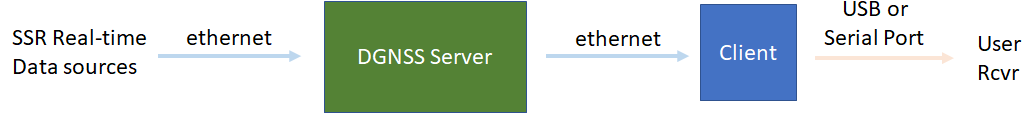
\includegraphics[scale=0.5]{./graphics/ClientServer}
	\caption{Client Server DGNSS Architecture. }
	\label{fig:ClientServer}
\end{figure}

\section{Client}
In the following sections we outline compilation, installation, GPS receiver setup, and execution of the \texttt{WADGNSS\_Client} application. 
We assume most users will read the guide sequentially once and then use it only as a reference document.

We recommend that most users begin from the \textbf{Installation} subsection, which describes the procedure for installing a pre-compiled executable application. 
We also distribute the source code.
Users who wish to start from the source code to compile the \texttt{WADGNSS\_Client} application should begin in the \textbf{Compilation} subsection. 

\subsection{Client Software Compilation}
The following procedure outlines compilation on the Ubuntu 18.04 operating system. The procedure may be compatible with other Linux distributions, but is untested as we are actively developing on Ubuntu.

\begin{enumerate}
\item Download the necessary prerequisite software to compile \texttt{WADGNSS\_Client} source. You will need the \texttt{cmake} build tool and a \texttt{C++} compiler such as \texttt{g++}. If not already installed on your local system, you can run the following commands to download the most recent releases.
\begin{verbatim}
$ sudo apt update && sudo apt upgrade 
$ sudo apt clean && sudo apt auto-remove 
$ sudo apt install make cmake g++ 
\end{verbatim}

\item Compile the client software on your local machine.

\begin{enumerate}
\item Navigate to the \texttt{WADGNSS\_Client} root directory. The root directory contains a \texttt{CMakeLists.txt} file.

\item Execute the following to make a build directory and navigate into the newly created build directory. 
\begin{verbatim}
$ mkdir build && cd build 
\end{verbatim}

\item Compile the \texttt{WADGNSS\_Client} by executing the following commands. The first command will configure the \texttt{cmake} build system and the second will invoke \texttt{make} to start the compilation process.
\begin{verbatim}
$ cmake .. && make 
\end{verbatim}

\item If compilation is successful an executable named \texttt{WADGNSS\_Client} will be visible in the build directory. The client software is now successfully compiled.
\end{enumerate}
\end{enumerate}
\noindent
You can now proceed to Section \ref{sect:RcvrSetup}. 
 
 
\subsection{Client Software Installation}
This section describes the recommended installation procedure for the \texttt{WADGNSS\_Client} executable. 
At present, we support installation on Ubuntu 18.04 (\href{https://releases.ubuntu.com/18.04/}{Ubuntu 18.04.5 LTS}). However, we are working to provide support for other operating systems and are focusing our efforts on releasing a Windows compatible client soon. 

\begin{enumerate}
\item In any directory on your machine create a new directory and  navigate into the new directory with the following command.
\begin{verbatim}
$ mkdir WADGNSS && cd WADGNSS 
\end{verbatim}

\item Copy the \texttt{WADGNSS\_Client} executable into the  \texttt{WADGNSS} directory. 
The \texttt{WADGNSS\_Client} executable is now successfully installed.
\end{enumerate}
You can now proceed to Section \ref{sect:RcvrSetup}.




\subsection{GPS Receiver Setup}\label{sect:RcvrSetup}
Before running the \texttt{WADGNSS\_Client} executable, the user must initialize and configure their receiver using its specific software or other interface. At present, \texttt{WADGNSS\_Client} software supports automated configuration for \href{module}{u-Blox ZED-F9P} and \href{module}{u-Blox M8P}. All other receivers need to be configured manually. Please note that \texttt{WADGNSS\_Client} currently only supports GPS receivers capable of serial input and output communications. Serial messages broadcast from a GPS receiver are used to serve corrections.

The following example on manual configuration is for a u-blox receiver using U-center. 
Manual configuration of other receivers can be accomplished by configuring the same parameters using the device specific configuration software:
\begin{itemize}
\item Enable GPS.
\item Disable all non-GPS navigation systems.
\item Enable PUBX 00 message in NMEA protocol.
\item Enable serial message output from the gps receiver. 
\item Enable RTCM version 3 serial message input.
\end{itemize}

An example for u-blox receivers using U-center software is shown below.

Step 1: Enable GPS and set GPS only.
 

Go to \emph{View} $\rightarrow$ \emph{Messages View} $\rightarrow$ \emph{UBX} $\rightarrow$ \emph{GNSS}. Select enable GPS and disable others. Then click "\emph{Send}"
\begin{figure}[H]
	\centering
	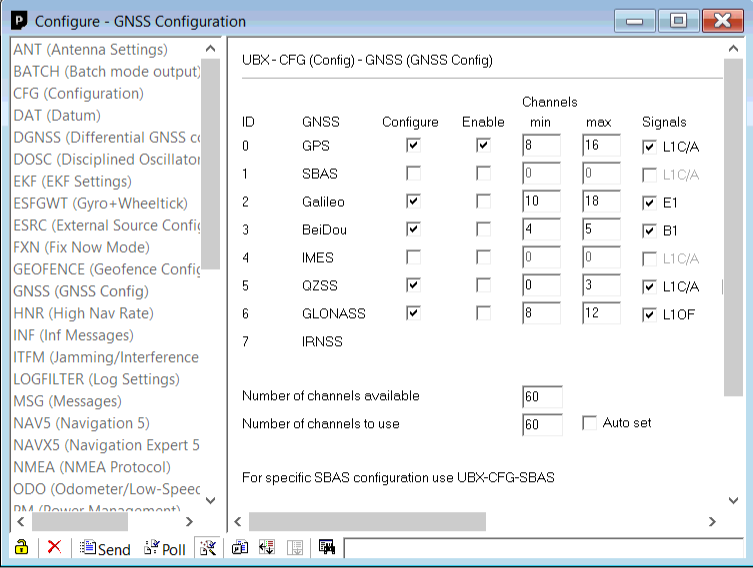
\includegraphics[scale=0.5]{./graphics/gnssset}
	\caption{Step 1 \label{fig:gnss}}
\end{figure}

Step 2: Enable PUBX 00 via NMEA protocol. 


Go to \emph{View} $\rightarrow$ \emph{Messages View} $\rightarrow$ \emph{NMEA} $\rightarrow$ \emph{PUBX}. Right click "\emph{00}" then select "\emph{Enable Message}".
\begin{figure}[H]
	\centering
	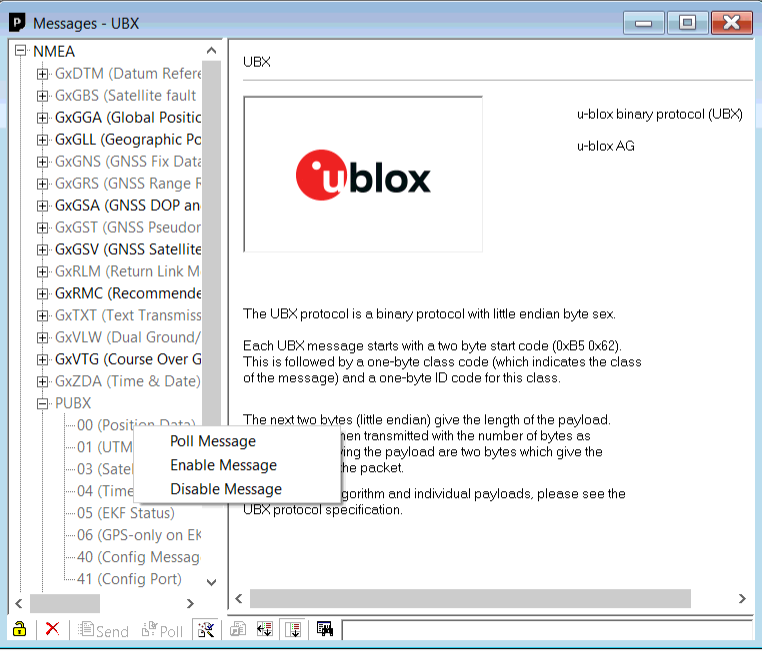
\includegraphics[scale=0.4]{./graphics/pubx00}
	\caption{Step 2 \label{fig:pubx}}
\end{figure}

Step 3: Enable a receiver USB port for RTCM version 3 input. 


Go to \emph{View} $\rightarrow$ \emph{Messages View} $\rightarrow$ \emph{UBX} $\rightarrow$ \emph{CFG} $\rightarrow$ \emph{CFG} $\rightarrow$ \emph{PRT}. Select the options based on Fig. \ref{fig:usb}. Then click "\emph{Send}". 
\begin{figure}[H]
	\centering
	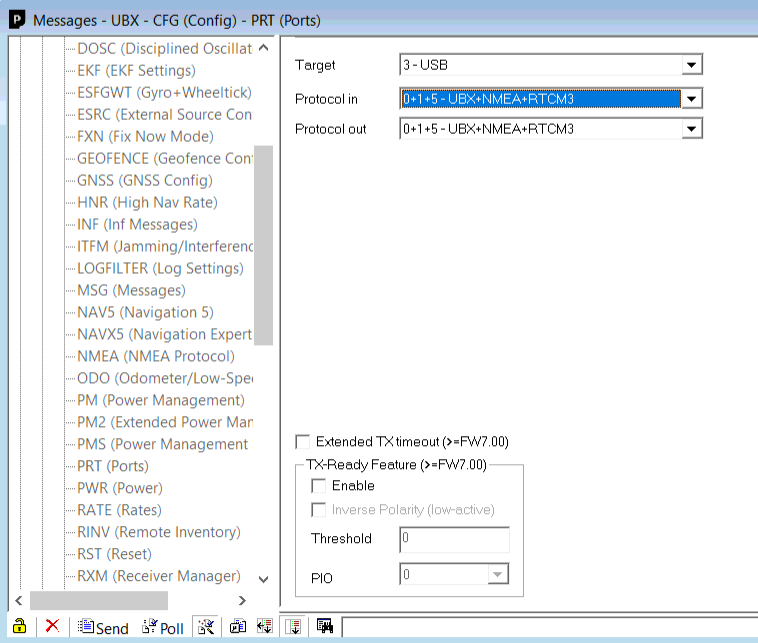
\includegraphics[scale=0.4]{./graphics/usb}
	\caption{Step 3 \label{fig:usb}}
\end{figure}

We recommend saving the configuration to the gps receiver. If configurations are saved the receiver should remain configured the next time it starts following power off. In U-center, configurations can be saved to the gps receiver by navigating to the \emph{CFG}  menu item on the \emph{Configuration View}. Then, select \emph{Save current configuration}. Finally, press the \emph{Send} button. The configurations will save to the receiver. Unfortunately, steps for saving configurations in other gps receiver configuration software will differ. 

\subsection{\texttt{WADGNSS\_Client} Execution}
The \texttt{WADGNSS\_Client} executable expects four command line arguments: com port, configuration option, server IP and server port. An example usage template is shown below. 
\begin{verbatim}
$ ./WADGNSS_Client [com port] [configuration] [server IP] [server port]
\end{verbatim}
The following sections discuss these command line parameters and how to find the correct values for your system. 

\subsubsection{\texttt{[com port]} Paramater}
The \texttt{[com port]} option designates on which of the computers \texttt{USB} communication ports the \texttt{WADGNSS\_Client} software receive messages from the GPS receiver. 
Determining port number to which the GPS receiver is broadcasting is operating system specific.
It may take a couple attempts to discover the correct filepath. 

In Ubuntu, serial data from the GPS receiver is available at a filepath matching the pattern \texttt{\textbackslash dev\textbackslash ttyACMX} where \texttt{X} is a number in the range [0-9]. For example, data from our receiver might be available at \texttt{\textbackslash dev\textbackslash ttyACM0} so we provide the filepath \texttt{\textbackslash dev\textbackslash ttyACM0} in place of the \texttt{[com port]} argument.

In Windows, the com port can be determined by opening \texttt{Device Manager} and expanding \texttt{Ports (COM \& LPT)} option. For example, suppose your GPS receiver is visible as device \texttt{COM6}. Then, the filepath \texttt{COM6} is provided in place of the \texttt{[com port]} argument.

\subsubsection{\texttt{[configuration] Paramater}}
The \texttt{[configuration]} parameter indicates the desired configuration of the supported GPS receiver. If supported, the \texttt{WADGNSS\_Client} will initialize the connected GPS receiver to the corresponding configuration. We currently support these automated configuration options:
\begin{itemize}
\item 0: Receiver configured by its software,
\item 1: u-blox M8P module
\item 2: u-blox ZED-F9P module
\end{itemize}

\subsubsection{\texttt{[server IP]} and \texttt{[server port]} Parameters}
The \texttt{[server IP]} and \texttt{[server port]} parameters indicate the network location of the  \texttt{WADGNSS\_Server} to which the \texttt{WADGNSS\_Client} will connect. 
We recommed connecting to the official WADGNSS server hosted at IP address \green write IP address here\black on port \green write port here \black . Substitue these values for \texttt{[server IP]} and \texttt{[server port]} paramaters when executing the \texttt{WADGNSS\_Client}, respectively.

\subsubsection{Example Execution}

Bringing all this  together, an example execution command for the \texttt{WADGNSS\_Client} where \texttt{USB} data is available at \texttt{\textbackslash dev\textbackslash ttyACM0}, the connected GNSS receiver is u-blox M8P, and the client will connect to a \texttt{WADGNSS\_Server} at IP \texttt{63.45.125.1} on port \texttt{8772} is as follows:
%
\begin{verbatim}
$ WADGNSS_Client \dev\ttyACM0 1 63.45.125.1 8772 
\end{verbatim}
%
Congratulations you have successfully launched the \texttt{WADGNSS\_Client}. To stop the \texttt{WADGNSS\_Client} press "ctrl + c" keys, simultaneously.

\end{document}
